% ============================================================
% RESEARCH PROPOSAL --- IEEE Two-Column Compact Style
% Digital Financial Transaction Fraud Detection Using
% Explainable Multi-Model Machine Learning on PaySim and IEEE-CIS
% ============================================================
\documentclass[10pt,a4paper,twocolumn]{article}

% --- Packages ---
\usepackage[utf8]{inputenc}
\usepackage{algorithm}
\usepackage{algpseudocode}
\usepackage[T1]{fontenc}
\usepackage{mathptmx}
\usepackage[left=1.8cm,right=1.8cm,top=2cm,bottom=2cm]{geometry}
\usepackage{setspace}
\usepackage{graphicx}
\usepackage{booktabs}
\usepackage{tabularx}
\usepackage{array}
\usepackage{multirow}
\usepackage{amsmath,amssymb}
\usepackage{enumitem}
\usepackage{hyperref}
\usepackage{xcolor}
\usepackage{tikz}
\usetikzlibrary{shapes.geometric, arrows.meta, positioning, fit, calc, backgrounds}
\usepackage{caption}
\usepackage{float}
\usepackage{titlesec}
\usepackage{fancyhdr}
\usepackage{balance}

% --- Color Palette ---
\definecolor{ieeeblue}{HTML}{1F4E79}
\definecolor{absbox}{HTML}{E8F0FE}
\definecolor{hypbox}{HTML}{FFF3E0}
\definecolor{secline}{HTML}{2E75B6}
\definecolor{citeblue}{HTML}{2962A0}
\definecolor{notebox}{HTML}{E8F5E9}
\definecolor{warnbox}{HTML}{FFF8E1}

% --- Compact Formatting ---
\singlespacing
\setlength{\parindent}{0pt}
\setlength{\parskip}{3pt}
\setlength{\columnsep}{0.6cm}
\setlist{nosep,leftmargin=*,topsep=1pt}
\captionsetup{font=small,skip=3pt,labelfont=bf}

\hypersetup{
    colorlinks=true,
    linkcolor=ieeeblue,
    citecolor=citeblue,
    urlcolor=ieeeblue,
}

% --- Section Formatting ---
\titleformat{\section}
  {\normalsize\bfseries\scshape\color{ieeeblue}}
  {\Roman{section}.}{0.4em}{}
  [\vspace{-2pt}{\color{secline}\titlerule[0.8pt]}]
\titleformat{\subsection}
  {\small\bfseries}
  {\arabic{section}.\arabic{subsection}}{0.4em}{}
\titlespacing*{\section}{0pt}{8pt}{4pt}
\titlespacing*{\subsection}{0pt}{6pt}{2pt}

% --- Header ---
\pagestyle{fancy}
\fancyhf{}
\renewcommand{\headrulewidth}{0pt}
\fancyfoot[C]{\small\thepage}

% ============================================================
\begin{document}

% --- Title Block ---
\twocolumn[{%
\begin{center}
    {\footnotesize\color{gray} RESEARCH PROPOSAL --- FINANCIAL TECHNOLOGY}\par\vspace{4pt}
    {\Large\bfseries\color{ieeeblue} Digital Financial Transaction Fraud Detection Using\par\vspace{2pt}
    Explainable Multi-Model Machine Learning\par\vspace{2pt}
    on PaySim and IEEE-CIS}\par\vspace{8pt}
    {\small Author~1\textsuperscript{1}, Author~2\textsuperscript{1}, Author~3\textsuperscript{1}, Author~4\textsuperscript{1}}\par\vspace{2pt}
    {\footnotesize\textsuperscript{1}Faculty of Information Technology, [University Name]}\par\vspace{1pt}
    {\footnotesize\texttt{\{author1, author2, author3, author4\}@university.edu}}\par\vspace{4pt}
    {\small\today}\par\vspace{6pt}
\end{center}
% --- Abstract Box ---
\noindent\fcolorbox{ieeeblue}{absbox}{%
\begin{minipage}{0.96\textwidth}
\vspace{4pt}
{\small\textbf{\color{ieeeblue}Abstract.}
This proposal presents the \textbf{Multi-View Stacking Ensemble with Explainable AI (MVS-XAI)} framework for financial fraud detection. The architecture integrates five base models---Random Forest, XGBoost, LightGBM, LSTM, and Graph Attention Network---each receiving \textbf{distinct input representations} (flat tabular features, account-level temporal sequences, and transaction subgraphs) to achieve diversity through data representation rather than algorithm selection alone. Class imbalance (1.3--3.5\% fraud rate) is addressed via K-Means SMOTE (data-level) and Focal Loss (algorithm-level for DL models). A Logistic Regression meta-learner combines out-of-fold predictions generated through \textbf{5-block walk-forward} temporal cross-validation, while a \textbf{four-level XAI system} (SHAP, LIME, DiCE, Anchors) ensures regulatory-compliant decision transparency with measurable quality metrics. The framework is validated on \textbf{dual benchmarks}---PaySim (6.3M transactions) and IEEE-CIS (590K transactions)---with leakage-safe temporal splitting, empirical ablation study, and McNemar's statistical testing with Holm correction.}
\vspace{4pt}
\end{minipage}%
}%
\par\vspace{2pt}
{\small\textbf{Keywords:} fraud detection, multi-view learning, stacking ensemble, explainable AI, class imbalance, graph attention network}
\par\vspace{6pt}
}]% end twocolumn

% ============================================================
% I. INTRODUCTION
% ============================================================
\section{Introduction}

\subsection{Background of the Study}

Global digital payment volumes surpassed \$11.6 trillion in 2024 \cite{statista2024}, accompanied by increasingly sophisticated fraud. Organizations lose approximately 5\% of annual revenue to fraud \cite{acfe2024}. Traditional rule-based detection relies on static thresholds and cannot adapt to evolving criminal strategies \cite{abdallah2016}. Machine learning (ML) has emerged as the dominant paradigm, with gradient boosted decision trees (XGBoost, LightGBM) representing the current state-of-the-art for tabular fraud detection \cite{chen2016, ke2017}.

However, existing ML approaches exhibit three critical limitations. First, most ensemble systems combine models from a single paradigm (e.g., multiple tree-based models), resulting in correlated predictions that provide diminishing stacking benefit \cite{dietterich2000}. Second, ``black-box'' models conflict with regulatory mandates such as GDPR Article~22 and the EU AI Act \cite{goodman2017}. Third, most studies validate on a single dataset, providing limited generalizability evidence.

\subsection{Research Problem}

Three gaps persist in the literature:

\begin{enumerate}
    \item \textbf{Limited input representation diversity:} Most ensembles feed the same flat feature matrix to all models. Research shows that diversity from \emph{different data representations} (tabular, temporal, graph) provides stronger complementarity than algorithm diversity alone \cite{dietterich2000}.
    \item \textbf{Insufficient explainability:} Existing work employs at most one XAI technique, providing incomplete transparency for regulators and investigators.
    \item \textbf{Narrow validation:} Single-dataset evaluations provide no cross-domain generalizability evidence. Concept drift further challenges model reliability over time \cite{santos2018}.
\end{enumerate}

\subsection{Research Objectives and Research Questions}

\begin{table}[H]
\centering
{\small
\begin{tabularx}{\columnwidth}{@{}lX@{}}
\toprule
\textbf{Obj.} & \textbf{Description / Research Question} \\
\midrule
O1 & Design a multi-view stacking ensemble with three input representations. \\
   & \textit{RQ1: Does multi-view stacking significantly outperform single-view ensembles?} \\[2pt]
O2 & Develop a 4-level XAI framework for comprehensive interpretability. \\
   & \textit{RQ2: Can the 4-level XAI satisfy regulatory transparency requirements?} \\[2pt]
O3 & Validate on dual benchmarks (PaySim and IEEE-CIS) with temporal splitting. \\
   & \textit{RQ3: Does $\Delta$F1 $\leq 0.10$ hold across domains?} \\[2pt]
O4 & Quantify each model's marginal contribution via empirical ablation with statistical testing. \\
   & \textit{RQ4: Which input representation contributes most to fraud detection?} \\
\bottomrule
\end{tabularx}
}
\end{table}

\subsection{Research Motivation and Contribution}

This study contributes: (1)~the \textbf{Multi-View Stacking Ensemble (MVS-XAI)} framework that achieves diversity through distinct input representations---flat tabular, temporal sequences, and transaction graphs---rather than relying solely on algorithm diversity; (2)~the \textbf{most comprehensive XAI coverage} in fraud detection (four complementary levels); (3)~\textbf{dual-benchmark validation} with temporal splitting and McNemar's statistical testing; and (4)~\textbf{rigorous empirical ablation} measuring actual prediction correlation rather than theoretical diversity assumptions.

% ============================================================
% II. LITERATURE REVIEW
% ============================================================
\section{Literature Review and Hypothesis Development}

\subsection{Literature Review}

\subsubsection{Tree-Based Ensemble Methods}

Gradient boosted decision trees remain the gold standard for tabular fraud detection. XGBoost achieves superior recall through sequential error correction \cite{chen2016}; LightGBM offers efficiency via leaf-wise growth for large-scale datasets \cite{ke2017}; Random Forest provides robust variance reduction through bagging \cite{breiman2001}. Grinsztajn et~al. \cite{grinsztajn2022} confirmed at NeurIPS 2022 that tree-based models consistently outperform standard deep learning on tabular data, reinforcing their role as baselines.

Wolpert's stacked generalization \cite{wolpert1992} provides the theoretical foundation for combining learners. Dietterich \cite{dietterich2000} showed that ensemble diversity drives performance gain. However, Kuncheva and Whitaker \cite{kuncheva2003} cautioned that no single diversity metric reliably predicts ensemble accuracy---suggesting that \emph{empirical measurement} of prediction correlation is essential rather than relying on theoretical diversity claims.

\subsubsection{Temporal and Graph-Based Approaches}

\textbf{LSTM for Sequential Fraud Patterns.} While standard LSTM performs poorly on flat tabular data \cite{jurgovsky2018}, research demonstrates that LSTMs ``offer significant advantages when data contains sequential and temporal dependencies''---capturing behavioral anomalies (e.g., rapid successive transactions) that tree models require extensive hand-crafted features to detect. Hybrid architectures combining trees (for static features) with LSTMs (for behavioral sequences) consistently outperform either approach alone.

\textbf{Graph Neural Networks} model transactions as networks, excelling at detecting coordinated fraud rings \cite{liu2021}. Graph Attention Networks (GAT) \cite{velickovic2018} weight neighbor importance via attention, but face scalability challenges on large graphs. NeighborLoader-based subgraph sampling \cite{hamilton2017} enables mini-batch training on millions of nodes, making GNNs practical for PaySim-scale datasets. Recent work on temporal GNNs---including CaT-GNN \cite{catgnn2024} for causal-temporal reasoning and TeMP-TraG \cite{tempgraph2024} for edge-based temporal message passing---demonstrates that incorporating temporal dynamics into graph message passing significantly improves fraud detection robustness.

\textbf{Why Not Transformers for Tabular Data?} While TabNet and FT-Transformer have emerged as competitive deep learning alternatives for tabular classification, Grinsztajn et~al. \cite{grinsztajn2022} systematically demonstrated at NeurIPS 2022 that tree-based models consistently outperform deep learning on medium-sized tabular datasets with heterogeneous features---a finding corroborated by extensive benchmarking. We therefore adopt trees for the tabular view but reserve DL architectures (LSTM, GAT) for sequential and graph views, where their inductive biases (recurrence, attention over neighborhoods) are well-matched to the data structure.

\subsubsection{Explainable AI in Finance}

The XAI literature identifies four complementary explanation families: (1)~SHAP for global feature attribution via Shapley values \cite{lundberg2017}; (2)~LIME for instance-level surrogate models \cite{ribeiro2016}; (3)~DiCE for counterfactual ``what-if'' scenarios with domain constraints \cite{mothilal2020}; (4)~Anchors for high-precision if-then rules suitable for regulatory reports \cite{ribeiro2018}. No prior fraud detection study integrates all four levels.

\subsubsection{Class Imbalance and Validation}

Fraud datasets exhibit extreme imbalance ($<$5\% positive). K-Means SMOTE \cite{last2017} has shown superior performance over standard SMOTE \cite{chawla2002} and SMOTE-ENN by clustering the minority class before generating synthetic samples, avoiding blind generation in noisy regions. Critically, resampling must occur \emph{within} each cross-validation fold to prevent data leakage \cite{santos2018}. Furthermore, temporal train-test splitting is essential---random splits leak future information, producing over-optimistic estimates.

\subsubsection{Research Gap Summary}

Table~\ref{tab:gap} synthesizes the limitations of existing approaches and positions this study's contributions.

\begin{table}[H]
\centering
\caption{Positioning against existing fraud detection approaches.}
\label{tab:gap}
{\scriptsize
\begin{tabularx}{\columnwidth}{@{}lcccc@{}}
\toprule
\textbf{Characteristic} & \textbf{Tree} & \textbf{DL} & \textbf{GNN} & \textbf{Ours} \\
 & \textbf{Ens.} & \textbf{Hybrid} & \textbf{Only} & \textbf{(MVS-XAI)} \\
\midrule
Multi-view input  & \texttimes & $\sim$ & \texttimes & \checkmark \\
Temporal + Graph   & \texttimes & \texttimes & \checkmark & \checkmark \\
4-level XAI        & \texttimes & \texttimes & \texttimes & \checkmark \\
Dual-benchmark     & \texttimes & $\sim$ & \texttimes & \checkmark \\
Temporal CV        & $\sim$ & $\sim$ & \texttimes & \checkmark \\
Statistical test   & \texttimes & \texttimes & \texttimes & \checkmark \\
\bottomrule
\end{tabularx}
}
\vspace{2pt}
{\scriptsize\textit{Note:} \checkmark = fully addressed, $\sim$ = partially addressed, \texttimes = not addressed. ``Tree Ens.'' covers XGBoost/LGBM stacking studies; ``DL Hybrid'' covers LSTM+tree studies; ``GNN Only'' covers GAT/GCN fraud studies.}
\end{table}

\subsection{Hypothesis Development}

\noindent\fcolorbox{orange!70!black}{hypbox}{%
\begin{minipage}{0.95\columnwidth}
\vspace{3pt}
{\small
\textbf{H1:} The multi-view stacking ensemble achieves significantly higher PR-AUC (primary) and F1 than any individual model ($p < 0.05$, exact McNemar with Holm-adjusted pairwise comparisons) \cite{wolpert1992}.\par\vspace{2pt}
\textbf{H2:} Multi-view stacking (tabular + temporal + graph) outperforms single-view stacking (tabular-only), confirming input representation diversity is more effective than algorithm diversity alone.\par\vspace{2pt}
\textbf{H3:} Cross-dataset $\Delta$F1 $\leq 0.10$, demonstrating domain generalizability.\par\vspace{2pt}
\textbf{H4:} The 4-level XAI achieves measurable quality: attribution faithfulness (deletion/insertion AUC), counterfactual validity $>$90\%, and anchor precision $>$90\% while preserving practical coverage \cite{lundberg2017}.
}
\vspace{3pt}
\end{minipage}%
}

% ============================================================
% III. DATA AND METHODOLOGY
% ============================================================
\section{Data and Methodology}

\subsection{Conceptual Framework}

\subsubsection{Multi-View Design Principle}

The framework's core innovation is achieving diversity through \textbf{distinct input representations} rather than relying solely on algorithm diversity:

\begin{enumerate}
    \item \textbf{Tabular View} (flat feature matrix): Engineered domain features fed to tree models (RF, XGBoost, LightGBM).
    \item \textbf{Sequential View} (temporal sequences): Account-level transaction sequences fed to LSTM.
    \item \textbf{Graph View} (transaction subgraph): Account relationship graph fed to GAT.
\end{enumerate}

Each view captures fundamentally different fraud signals---static patterns, behavioral anomalies, and relational structures---providing stronger complementarity than multiple models trained on the same feature matrix. Prediction correlation is \textbf{measured empirically} via OOF outputs rather than assumed theoretically.

\subsubsection{Research Pipeline}

Figure~\ref{fig:pipeline} presents the end-to-end pipeline with six stages.

\begin{figure}[H]
\centering
\resizebox{\columnwidth}{!}{
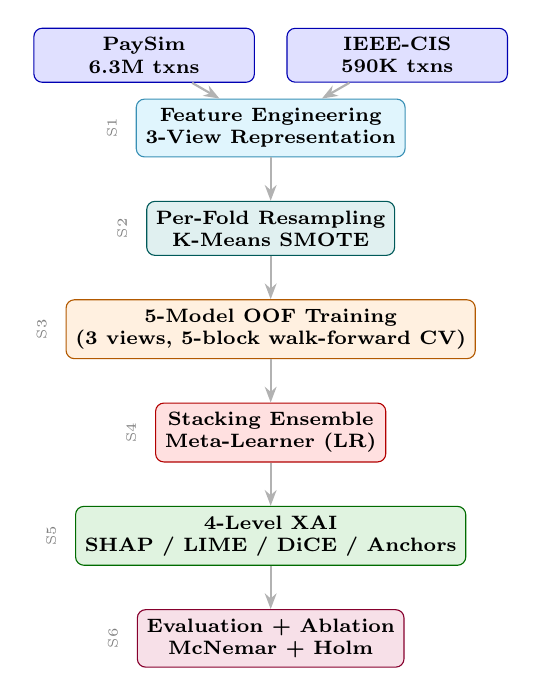
\begin{tikzpicture}[
    node distance=0.45cm,
    every node/.style={font=\scriptsize},
    phase/.style={rectangle, rounded corners=3pt, draw=#1!70!black, fill=#1!12,
                  minimum width=2.8cm, minimum height=0.6cm, align=center,
                  font=\scriptsize\bfseries},
    arr/.style={-{Stealth[length=2mm]}, thick, color=gray!60},
]
    \node[phase=blue] (d1) {PaySim\\6.3M txns};
    \node[phase=blue, right=0.4cm of d1] (d2) {IEEE-CIS\\590K txns};

    \node[phase=cyan, below=0.55cm of $(d1)!0.5!(d2)$] (pp) {Feature Engineering\\3-View Representation};

    \node[phase=teal, below=0.55cm of pp] (rs) {Per-Fold Resampling\\K-Means SMOTE};

    \node[phase=orange, below=0.55cm of rs] (ml) {5-Model OOF Training\\(3 views, 5-block walk-forward CV)};

    \node[phase=red, below=0.55cm of ml] (opt) {Stacking Ensemble\\Meta-Learner (LR)};

    \node[phase=green!60!black, below=0.55cm of opt] (xai) {4-Level XAI\\SHAP / LIME / DiCE / Anchors};

    \node[phase=purple, below=0.55cm of xai] (ev) {Evaluation + Ablation\\McNemar + Holm};

    \draw[arr] (d1) -- (pp);
    \draw[arr] (d2) -- (pp);
    \draw[arr] (pp) -- (rs);
    \draw[arr] (rs) -- (ml);
    \draw[arr] (ml) -- (opt);
    \draw[arr] (opt) -- (xai);
    \draw[arr] (xai) -- (ev);

    \node[left=0.12cm of pp, font=\tiny, text=gray, rotate=90, anchor=south] {S1};
    \node[left=0.12cm of rs, font=\tiny, text=gray, rotate=90, anchor=south] {S2};
    \node[left=0.12cm of ml, font=\tiny, text=gray, rotate=90, anchor=south] {S3};
    \node[left=0.12cm of opt, font=\tiny, text=gray, rotate=90, anchor=south] {S4};
    \node[left=0.12cm of xai, font=\tiny, text=gray, rotate=90, anchor=south] {S5};
    \node[left=0.12cm of ev, font=\tiny, text=gray, rotate=90, anchor=south] {S6};
\end{tikzpicture}
}
\caption{End-to-end research pipeline with six stages.}
\label{fig:pipeline}
\end{figure}


\subsection{Data Description}

Table~\ref{tab:datasets} summarizes both datasets. The \emph{same architecture} is applied independently to each; results are compared side-by-side.

\begin{table}[H]
\centering
\caption{Benchmark dataset characteristics.}
\label{tab:datasets}
{\small
\begin{tabularx}{\columnwidth}{lXX}
\toprule
\textbf{Property} & \textbf{PaySim} & \textbf{IEEE-CIS} \\
\midrule
Domain & Mobile money & E-commerce \\
Transactions & 6,362,620 & 590,540 \\
Fraud rate & 1.29\% & 3.50\% \\
Features & 11 (interpretable) & 434 (partially masked) \\
Source & Synthetic \cite{lopezrojas2016} & Real \cite{ieee2019} \\
Key challenge & Scale; 2 fraud types & 40\% missing values \\
Temporal field & \texttt{step} (hourly) & \texttt{TransactionDT} \\
\bottomrule
\end{tabularx}
}
\end{table}

\subsection{Research Methods}

\subsubsection{Multi-View Stacking Architecture}

The framework operates in two levels, as shown in Figure~\ref{fig:architecture}. Five base models spanning three input views produce out-of-fold (OOF) predictions via 5-block walk-forward cross-validation with temporal gap.

\textbf{Level~1 --- Base Models:}

\begin{enumerate}
    \item \textbf{Random Forest} \cite{breiman2001} (Tabular, Bagging): 500 trees, \texttt{class\_weight='balanced\_subsample'}\footnote{Unlike \texttt{'balanced'} which computes weights once on the full training set, \texttt{'balanced\_subsample'} recomputes class weights per bootstrap sample, adapting to each tree's specific data subset.}, \texttt{max\_features='sqrt'}. Provides variance reduction complementary to boosting.
    \item \textbf{XGBoost} \cite{chen2016} (Tabular, Boosting): 1000 rounds with early stopping, \texttt{scale\_pos\_weight} $= N_{neg}/N_{pos}$, L1/L2 regularization. Sequential error correction on all features.
    \item \textbf{LightGBM} \cite{ke2017} (Tabular, Boosting): leaf-wise growth, \texttt{is\_unbalance=True}. Efficient on large-scale PaySim dataset.
    \item \textbf{LSTM} (Sequential, Deep Learning): 2-layer, 128 hidden units, dropout=0.3. Trained with \textbf{Focal Loss} \cite{lin2017} ($\gamma{=}2$, $\alpha{=}0.75$) to focus on hard-to-detect fraud patterns (e.g., structuring, account takeover) rather than easy majority examples. Receives \textbf{temporal sequences} (View~2)---not flat features.
    \item \textbf{GAT} \cite{velickovic2018} (Graph, GNN): 2-layer, 8 attention heads, hidden=64. Focal Loss ($\gamma{=}2$, $\alpha{=}0.75$). Operates on \textbf{transaction subgraphs} (View~3) via NeighborLoader. Detects coordinated fraud rings invisible to tabular models.
\end{enumerate}

\textbf{Level~2 --- Meta-Learner.} Logistic Regression (L2, $C$=1.0, \texttt{class\_weight='balanced'}) combines the five OOF probability vectors plus two \texttt{view\_mask} binary indicators (\texttt{view\_mask\_seq}, \texttt{view\_mask\_graph}), yielding a 7-dimensional input. LR is chosen because: (a)~the input is low-dimensional (7 features), making complex meta-learners prone to overfitting; (b)~LR coefficients provide directly interpretable model contribution weights; (c)~LR outputs well-calibrated probabilities suitable for threshold optimization; (d)~L2 regularization prevents any single base model from dominating. Soft Voting (average) serves as an ablation baseline.

\textbf{Loss Strategy.} Table~\ref{tab:loss} summarizes the loss design. The guiding principle is to match loss complexity to model complexity: tree-based models already focus on hard examples through residual-based boosting, so simple weighted loss suffices; deep learning models require Focal Loss because standard BCE is dominated by the 98.7\% majority class.

\begin{table}[H]
\centering
\caption{Loss function design per model.}
\label{tab:loss}
{\small
\begin{tabularx}{\columnwidth}{@{}lXll@{}}
\toprule
\textbf{Model} & \textbf{Loss} & \textbf{Imbalance} & \textbf{Hard Ex.} \\
\midrule
RF & Weighted Gini & balanced\_sub. & Bagging \\
XGBoost & Weighted Log & scale\_pos\_wt & Residuals \\
LightGBM & Weighted Log & is\_unbalance & Residuals \\
LSTM & \textbf{Focal Loss} & $\alpha{=}0.75$ & $\gamma{=}2$ \\
GAT & \textbf{Focal Loss} & $\alpha{=}0.75$ & $\gamma{=}2$ \\
Meta-LR & Log Loss + L2 & balanced & --- \\
\bottomrule
\end{tabularx}
}
\vspace{2pt}
{\scriptsize\textit{Note:} Focal Loss $FL(p_t) = -\alpha_t(1-p_t)^\gamma\log(p_t)$ \cite{lin2017}. For tree models, boosting's sequential residual fitting inherently addresses hard examples, making Focal Loss unnecessary and potentially destabilizing.}
\end{table}

\textbf{Probability Calibration.} Since the meta-learner receives heterogeneous model probabilities, calibration quality directly impacts stacking performance. Calibrators are fitted on \emph{out-of-fold validation predictions only} (never on the same samples used to fit base learners) to avoid biased calibration. We apply Isotonic Regression to LSTM/GAT probabilities by default, and to tree models if ECE remains high. Calibration quality is measured by ECE (with fixed binning protocol), Brier Score, and reliability diagrams.

\textbf{Decision Threshold Optimization.} Rather than using the default 0.5 threshold, we optimize the threshold $\tau^*$ to maximize the F2-Score on the validation set. F2 weights Recall twice as heavily as Precision, reflecting the asymmetric cost structure of fraud detection where false negatives (missed fraud) are far more costly than false positives.

\textbf{Hyperparameter Optimization.} Two-stage Optuna \cite{akiba2019} strategy: Stage~1 tunes each model on a blocked temporal split (200 TPE trials with MedianPruner and model-specific pruning callbacks). Stage~2 fixes best hyperparameters for full 5-block walk-forward OOF generation. Key search spaces include \texttt{learning\_rate} (log-scale), \texttt{max\_depth}, regularization terms, \texttt{scale\_pos\_weight}, and Focal Loss $\gamma \in \{1, 2, 3\}$.

\textbf{Leakage-Safe Experimental Protocol.} Algorithm~\ref{alg:protocol} formalizes the walk-forward pipeline ensuring no future information leaks into training.

\begin{algorithm}[H]
\caption{Leakage-Safe Walk-Forward OOF Protocol}
\label{alg:protocol}
{\small
\begin{algorithmic}[1]
\Require Dataset $\mathcal{D}$ sorted by timestamp, $K{=}5$ temporal blocks
\Ensure OOF predictions $\hat{p}^{\text{oof}}_m$ for each model $m$
\For{$k = 1$ \textbf{to} $K$}
    \State $\mathcal{T}_k \gets \mathcal{D}[t \leq t_{\text{end}}^{(k-1)}]$ \Comment{Train: all past blocks}
    \State $\mathcal{V}_k \gets \mathcal{D}[t_{\text{end}}^{(k-1)} + \text{gap} < t \leq t_{\text{end}}^{(k)}]$
    \State Fit encoders, scalers on $\mathcal{T}_k$ only; transform $\mathcal{V}_k$
    \State Apply K-Means SMOTE to $\mathcal{T}_k$ only (tabular view)
    \State Build temporal graph $G_k$ with edges $\{e : t_e \leq t_{\text{end}}^{(k-1)}\}$
    \For{each model $m \in \{\text{RF, XGB, LGBM, LSTM, GAT}\}$}
        \State Train $m$ on $\mathcal{T}_k$ (respective view)
        \State $\hat{p}^{\text{oof}}_m[\mathcal{V}_k] \gets m.\text{predict\_proba}(\mathcal{V}_k)$
    \EndFor
    \State Calibrate $\hat{p}^{\text{oof}}_{\text{LSTM}}, \hat{p}^{\text{oof}}_{\text{GAT}}$ via Isotonic on $\mathcal{V}_k$
\EndFor
\State Concatenate OOF: $X^{\text{meta}} \gets [\hat{p}^{\text{oof}}_1, \ldots, \hat{p}^{\text{oof}}_5, \texttt{view\_mask}]$
\State Train Meta-LR on $X^{\text{meta}}$
\end{algorithmic}
}
\end{algorithm}

% --- Architecture Diagram ---
\begin{figure*}[t]
\centering
\resizebox{0.92\textwidth}{!}{
\begin{tikzpicture}[
    node distance=0.4cm,
    every node/.style={font=\scriptsize},
    input/.style={rectangle, rounded corners=3pt, draw=blue!60!black, fill=blue!10,
                  minimum height=0.55cm, minimum width=1.4cm, align=center, font=\scriptsize\bfseries},
    view/.style={rectangle, rounded corners=3pt, draw=cyan!60!black, fill=cyan!8,
                 minimum height=0.55cm, minimum width=2.8cm, align=center, font=\scriptsize\bfseries},
    model/.style={rectangle, rounded corners=3pt, draw=#1!60!black, fill=#1!10,
                  minimum height=0.55cm, minimum width=1.65cm, align=center, font=\scriptsize\bfseries},
    meta/.style={rectangle, rounded corners=3pt, draw=red!60!black, fill=red!8,
                 minimum height=0.55cm, minimum width=4.5cm, align=center, font=\scriptsize\bfseries},
    xai/.style={rectangle, rounded corners=3pt, draw=green!50!black, fill=green!8,
                minimum height=0.55cm, minimum width=1.55cm, align=center, font=\scriptsize\bfseries},
    out/.style={rectangle, rounded corners=3pt, draw=purple!60!black, fill=purple!8,
                minimum height=0.55cm, minimum width=4.5cm, align=center, font=\scriptsize\bfseries},
    arr/.style={-{Stealth[length=1.8mm]}, semithick, color=gray!55},
    groupbox/.style={draw=#1!50, dashed, rounded corners=5pt, inner sep=5pt},
    plabel/.style={font=\tiny\itshape, text=gray!70},
]
    % --- Row 1: Two data sources ---
    \node[input] (d1) {PaySim};
    \node[input, right=1.8cm of d1] (d2) {IEEE-CIS};

    % --- Row 2: Three Views ---
    \node[view, below=0.8cm of $(d1)!0.5!(d2)$, xshift=-3.5cm] (v1) {View 1: Tabular\\{\tiny Flat feature matrix (N,F)}};
    \node[view, right=0.2cm of v1] (v2) {View 2: Sequential\\{\tiny Account sequences (N,T,F)}};
    \node[view, right=0.2cm of v2] (v3) {View 3: Graph\\{\tiny Transaction subgraph}};

    % --- Row 3: Five Base Models ---
    \node[model=orange, below=1.0cm of v1, xshift=-1.2cm] (rf) {RF\\{\tiny Bagging}};
    \node[model=orange, right=0.15cm of rf] (xgb) {XGBoost\\{\tiny Boosting}};
    \node[model=orange, right=0.15cm of xgb] (lgbm) {LightGBM\\{\tiny Boosting}};
    \node[model=violet, right=0.4cm of lgbm] (lstm) {LSTM\\{\tiny Seq. DL}};
    \node[model=teal, right=0.4cm of lstm] (gat) {GAT\\{\tiny Graph NN}};

    % --- Row 4: Meta-Learner ---
    \node[meta, below=1.0cm of $(rf)!0.5!(gat)$] (metalr) {Meta-Learner: Logistic Regression (L2) --- 5 OOF probabilities};

    % --- Row 5: Four XAI Methods ---
    \node[xai, below=1.0cm of metalr, xshift=-2.85cm] (shap) {SHAP\\{\tiny Global}};
    \node[xai, right=0.15cm of shap] (lime) {LIME\\{\tiny Local}};
    \node[xai, right=0.15cm of lime] (dice) {DiCE\\{\tiny Counterfact.}};
    \node[xai, right=0.15cm of dice] (anch) {Anchors\\{\tiny Rules}};

    % --- Row 6: Output ---
    \node[out, below=1.0cm of $(shap)!0.5!(anch)$] (output) {Explainable Fraud Decision + Audit Report};

    % --- Arrows: Data to Views (both datasets flow to all 3 views) ---
    \draw[arr] (d1.south) -- ++(0,-0.3) -| (v1.north);
    \draw[arr] (d1.south) -- ++(0,-0.3) -| (v2.north);
    \draw[arr] (d1.south) -- ++(0,-0.3) -| (v3.north);
    \draw[arr] (d2.south) -- ++(0,-0.3) -| (v1.north);
    \draw[arr] (d2.south) -- ++(0,-0.3) -| (v2.north);
    \draw[arr] (d2.south) -- ++(0,-0.3) -| (v3.north);

    % --- Arrows: Views to Models ---
    \draw[arr] (v1.south) -- ++(0,-0.25) -| (rf.north);
    \draw[arr] (v1.south) -- ++(0,-0.25) -| (xgb.north);
    \draw[arr] (v1.south) -- ++(0,-0.25) -| (lgbm.north);
    \draw[arr] (v2.south) -- ++(0,-0.25) -| (lstm.north);
    \draw[arr] (v3.south) -- ++(0,-0.25) -| (gat.north);

    % --- Arrows: Models to Meta ---
    \draw[arr] (rf.south) -- ++(0,-0.25) -| (metalr.north);
    \draw[arr] (xgb.south) -- ++(0,-0.25) -| (metalr.north);
    \draw[arr] (lgbm.south) -- ++(0,-0.25) -| (metalr.north);
    \draw[arr] (lstm.south) -- ++(0,-0.25) -| (metalr.north);
    \draw[arr] (gat.south) -- ++(0,-0.25) -| (metalr.north);

    % --- Arrows: Base Models to XAI (XAI is model-agnostic; each method can apply to any base model) ---
    % For clarity, we show primary assignments. In practice, all 4 XAI methods apply to all 5 models.
    % SHAP: TreeSHAP (trees), GradientSHAP (LSTM), GNNExplainer (GAT)
    \draw[arr, dashed, gray!40] (rf.south) -- ++(0,-0.65) -| (shap.north);
    \draw[arr, dashed, gray!40] (xgb.south) -- ++(0,-0.65) -| (shap.north);
    \draw[arr, dashed, gray!40] (lgbm.south) -- ++(0,-0.65) -| (lime.north);
    \draw[arr, dashed, gray!40] (lstm.south) -- ++(0,-0.65) -| (dice.north);
    \draw[arr, dashed, gray!40] (gat.south) -- ++(0,-0.65) -| (anch.north);
    % Meta-learner also connects to output for final decision
    \draw[arr] (metalr.south) -- ++(0,-0.25) -| ($(shap.north)!0.5!(anch.north)$);

    % --- Arrows: XAI to Output ---
    \draw[arr] (shap.south) -- ++(0,-0.25) -| (output.north);
    \draw[arr] (lime.south) -- ++(0,-0.25) -| (output.north);
    \draw[arr] (dice.south) -- ++(0,-0.25) -| (output.north);
    \draw[arr] (anch.south) -- ++(0,-0.25) -| (output.north);

    % --- Bounding Boxes ---
    \begin{scope}[on background layer]
        \node[groupbox=cyan, fit=(v1)(v2)(v3),
              label={[font=\tiny\bfseries\color{cyan!60!black}]above:Multi-View Input Representation}] {};
        \node[groupbox=orange, fit=(rf)(xgb)(lgbm)(lstm)(gat),
              label={[font=\tiny\bfseries\color{orange!70!black}]above:Level 1 --- 5 Base Models (5-block walk-forward OOF, K-Means SMOTE per fold)}] {};
        \node[groupbox=green, fit=(shap)(lime)(dice)(anch),
              label={[font=\tiny\bfseries\color{green!50!black}]above:4-Level XAI Framework}] {};
    \end{scope}

    % --- View annotations ---
    \node[plabel, below=0.02cm of rf, yshift=-0.15cm] {Tabular View};
    \node[plabel, below=0.02cm of lstm, yshift=-0.15cm] {Sequential View};
    \node[plabel, below=0.02cm of gat, yshift=-0.15cm] {Graph View};
    \node[right=0.1cm of metalr, font=\tiny, text=red!60!black] {\textit{Level 2}};
\end{tikzpicture}
}
\caption{Multi-View Stacking Ensemble with 4-Level XAI (MVS-XAI). Each view provides a fundamentally different representation of transaction data, achieving diversity through input representation rather than algorithm selection alone.}
\label{fig:architecture}
\end{figure*}

\subsubsection{Four-Level XAI Framework}

Each level targets a distinct stakeholder need. All four XAI methods are model-agnostic and are applied to \textbf{base models}, which operate on original features. The meta-learner (5 probability inputs) cannot provide meaningful feature-level explanations.

\begin{enumerate}
    \item \textbf{Global --- SHAP} \cite{lundberg2017}: TreeSHAP for exact Shapley values on RF/XGB/LGBM (polynomial time); GradientSHAP for LSTM; GNNExplainer for GAT---avoiding the prohibitive $O(2^F)$ cost of KernelSHAP on high-dimensional inputs. Produces global feature importance rankings and dependence plots for model auditing. \emph{``Which features drive fraud predictions overall?''}
    \item \textbf{Local --- LIME} \cite{ribeiro2016}: Per-transaction surrogate explanations applied to any base model flagging a transaction. Generates interpretable local feature weights for investigator alerts. \emph{``Why was this specific transaction flagged?''}
    \item \textbf{Counterfactual --- DiCE} \cite{mothilal2020}: Minimal feature changes to reverse prediction, with domain constraints (e.g., cannot change account age, transaction history). Applied primarily to tree models via the DiCE API. \emph{``What would make this transaction legitimate?''}
    \item \textbf{Rules --- Anchors} \cite{ribeiro2018}: High-precision if-then conditions extracted from any base model's decision boundary. \emph{``IF amount $>$ 200K AND full\_transfer THEN fraud (97\%).''} Most interpretable for non-technical regulators and compliance officers.
\end{enumerate}

\textbf{XAI Quality Measurement.} To make H4 testable, we report: (a) attribution faithfulness via deletion/insertion AUC and explanation stability across seeds; (b) counterfactual validity, proximity, and sparsity; (c) anchor precision and coverage. This avoids purely qualitative XAI claims.

\subsubsection{Evaluation Strategy}

Table~\ref{tab:metrics} presents evaluation metrics. Statistical significance is assessed via \textbf{exact McNemar's test} on paired predictions from the chronological test holdout, supplemented by Wilcoxon signed-rank tests on 5-block walk-forward CV results. Pairwise comparisons are reported with Holm-adjusted $p$-values.

\begin{table}[H]
\centering
\caption{Evaluation metrics for imbalanced fraud detection.}
\label{tab:metrics}
{\small
\begin{tabularx}{\columnwidth}{lX}
\toprule
\textbf{Metric} & \textbf{Rationale} \\
\midrule
F1-Score & Precision--Recall harmonic balance \\
F2-Score & Weighted toward Recall (cost of FN $\gg$ FP) \\
PR-AUC & \textbf{Primary} --- robust for extreme class imbalance \\
MCC & Balanced metric for skewed distributions \\
ECE + Brier & Probability calibration quality \\
McNemar/Wilcoxon & Significance testing (Holm-adjusted) \\
XAI quality & Faithfulness, counterfactual validity, anchor precision/coverage \\
\bottomrule
\end{tabularx}
}
\end{table}


% ============================================================
% IV. DATA PREPROCESSING
% ============================================================
\section{Data Preprocessing}


\subsection{Data Cleaning \& Variable Construction}

\subsubsection{Feature Engineering: Three-View Representation}

The core innovation lies in constructing three distinct input representations from the same raw transaction data, as summarized in Table~\ref{tab:views}.

\begin{table}[H]
\centering
\caption{Three-view input representation summary.}
\label{tab:views}
{\small
\begin{tabularx}{\columnwidth}{@{}lXll@{}}
\toprule
\textbf{View} & \textbf{Input Format} & \textbf{Fraud Signal} & \textbf{Models} \\
\midrule
Tabular & Flat matrix $(N, F)$ & Static anomalies (balance errors, large amounts) & RF, XGB, LGBM \\
Sequential & 3D tensor $(N, T, F)$ per account & Behavioral anomalies (rapid burst patterns) & LSTM \\
Graph & Node-edge structure & Relational patterns (fraud rings, shared devices) & GAT \\
\bottomrule
\end{tabularx}
}
\end{table}

\textbf{View~1: Tabular Features} (for RF, XGBoost, LightGBM). PaySim: balance error (\texttt{oldbalanceOrg $-$ amount $-$ newbalanceOrg}), amount-to-balance ratio, \texttt{is\_full\_transfer}, velocity features (rolling counts/amounts per account over 1h/6h/24h windows), and cyclical temporal encoding (hour sin/cos). IEEE-CIS: merge Transaction + Identity tables; impute missing values; target encoding for high-cardinality features; SHAP-based selection (434$\to$50--80). \textbf{Leakage control:} all encoders/statistics are fitted on each training fold only, then applied to validation/test. Graph-derived tabular features (degree, PageRank) are computed from \emph{fold-local past-only} transaction snapshots.

\textbf{View~2: Temporal Sequences} (for LSTM). Group transactions by account (\texttt{nameOrig} / \texttt{card1}), sort by time, create sliding windows of $T{=}10$ transactions. Each timestep encodes: amount, type, balance ratio, time delta, hour. Accounts with $<$3 transactions are excluded from LSTM---their OOF probability is replaced by the \emph{calibrated class prior} $P(\text{fraud}|\text{train\_fold}) \approx 0.013$, paired with a binary \texttt{view\_mask\_seq}$=0$ indicator. This ensures the meta-learner receives 5 probabilities for every sample while learning to discount masked views through the interaction between the prior and the mask feature (distinct from a simple zero-fill, which conflates ``confident legitimate'' with ``view unavailable''). Input shape: $(N_{\text{seq}}, T, F)$. The same calibrated-prior strategy applies to GAT when accounts lack sufficient graph neighborhood (\texttt{view\_mask\_graph}$=0$).

\textbf{View~3: Transaction Graph} (for GAT). Construct heterogeneous graph: nodes = accounts, edges = transactions. Node features: aggregated statistics (mean amount, transaction count, std). Edge features: amount, type, temporal delta. For PaySim (6.3M), use \texttt{NeighborLoader}(num\_neighbors=[10,5], batch=1024) for mini-batch training. For IEEE-CIS (590K), full graph may be feasible. \textbf{Temporal graph protocol:} within each split, only edges with timestamp $\leq t$ are visible for samples at time $t$, preventing future-edge leakage.

\noindent\fcolorbox{green!60!black}{notebox}{%
\begin{minipage}{0.95\columnwidth}
\vspace{2pt}
{\small\textbf{Key insight:} Each view captures fundamentally different fraud signals---tabular features capture static anomalies, temporal sequences capture behavioral drift, and graph structure captures coordinated fraud rings. This ``multi-view'' approach generates stronger diversity than feeding the same features to different algorithms.}
\vspace{2pt}
\end{minipage}%
}

\subsubsection{Data Splitting and Resampling}

\textbf{Temporal Splitting.} Train/validation/test sets are split \emph{chronologically}, not randomly (e.g., 70/15/15 by time)---ensuring the model never sees future transactions during training. This prevents over-optimistic estimates caused by random splitting in time-sensitive fraud detection.

\textbf{Time-Aware OOF Protocol.} OOF predictions are generated with 5-block \emph{walk-forward} CV (expanding window + gap). Each fold trains on past blocks and validates on the immediately following block, enforcing strict temporal causality.

\textbf{Resampling.} K-Means SMOTE is applied \emph{only to the training partition inside each fold} via \texttt{imblearn.pipeline.Pipeline} \cite{chawla2002}. Validation/test blocks remain untouched at original class distribution \cite{santos2018}.


% ============================================================
% V. EXPECTED RESULTS
% ============================================================
\section{Expected Results}

\subsection{Model Performance}

Table~\ref{tab:expected} presents anticipated performance based on published benchmarks \cite{chen2016, ke2017}. Estimates are conservative, reflecting realistic ranges from recent fraud detection literature (2023--2025).

\begin{table}[H]
\centering
\caption{Expected F1-Score and PR-AUC across benchmarks.}
\label{tab:expected}
{\small
\begin{tabular}{lcccc}
\toprule
& \multicolumn{2}{c}{\textbf{PaySim}} & \multicolumn{2}{c}{\textbf{IEEE-CIS}} \\
\cmidrule(lr){2-3} \cmidrule(lr){4-5}
\textbf{Model} & \textbf{F1} & \textbf{PR-AUC} & \textbf{F1} & \textbf{PR-AUC} \\
\midrule
RF (baseline)    & .895 & .870 & .828 & .800 \\
XGBoost          & .920 & .898 & .852 & .830 \\
LightGBM         & .918 & .892 & .856 & .838 \\
LSTM (temporal)  & .878 & .858 & .815 & .795 \\
GAT (graph)      & .865 & .845 & .802 & .785 \\
\midrule
Trees-only stack & .930 & .910 & .868 & .850 \\
\textbf{MVS-XAI (full)} & \textbf{.942} & \textbf{.922} & \textbf{.882} & \textbf{.865} \\
\bottomrule
\end{tabular}
}
\vspace{2pt}
{\scriptsize\textit{Note:} LSTM and GAT individually underperform trees on tabular benchmarks but contribute unique signals via temporal/graph views. Stacking improvement is modest ($+1$--$2\%$ per added view), consistent with recent fraud detection literature. All values are conservative estimates; actual results depend on feature engineering quality and dataset-specific characteristics.}
\end{table}

\subsection{Ablation Study Design}

The ablation study is organized into four groups addressing distinct research questions, all evaluated with PR-AUC (primary), F1, F2, MCC, and ECE (calibration error).

\textbf{Group~1: Multi-View Contribution.} Table~\ref{tab:ablation} tests the central thesis via incremental view addition with exact McNemar testing and Holm-adjusted pairwise comparisons.

\begin{table}[H]
\centering
\caption{Ablation: input view contribution to stacking (F1).}
\label{tab:ablation}
{\small
\begin{tabularx}{\columnwidth}{Xccl}
\toprule
\textbf{Configuration} & \textbf{PaySim} & \textbf{IEEE} & \textbf{Tests} \\
\midrule
XGBoost only (baseline)   & .920 & .852 & --- \\
Trees-only (RF+XGB+LGBM)  & .930 & .868 & single-view \\
\quad + LSTM (temporal)    & .934 & .874 & + seq.\ view \\
\quad + GAT (graph)        & .932 & .872 & + graph view \\
\quad + LSTM + GAT         & .942 & .882 & full multi-view \\
\midrule
Full (Soft Voting)         & .935 & .876 & vs.\ Stacking \\
\textbf{Full (Stacking)}   & \textbf{.942} & \textbf{.882} & \textbf{best} \\
\bottomrule
\end{tabularx}
}
\vspace{2pt}
{\scriptsize\textit{Note:} Improvements are incremental (1--2\% per added view), consistent with literature. Significance is reported with exact McNemar + Holm adjustment ($p<0.05$). Prediction correlation matrix will quantify actual diversity.}
\end{table}

\noindent\fcolorbox{orange!70!black}{warnbox}{%
\begin{minipage}{0.95\columnwidth}
\vspace{2pt}
{\small\textbf{Methodological note:} These are \emph{estimated} ranges. Actual prediction correlation between models will be \textbf{empirically measured} through OOF outputs---if any tree model shows $r > 0.95$ with another, the ablation study will report it as a finding rather than a pre-assumed conclusion \cite{kuncheva2003}.}
\vspace{2pt}
\end{minipage}%
}

\textbf{Group~2: Loss Function (LSTM/GAT).} Isolates the impact of Focal Loss versus alternatives on minority-class detection:
\begin{itemize}[nosep]
    \item \textit{L-1:} Standard BCE (baseline)
    \item \textit{L-2:} Weighted BCE ($\alpha{=}0.75$, $\gamma{=}0$ --- equivalent to class weighting only)
    \item \textit{L-3:} Focal Loss ($\gamma{=}1$, mild focusing)
    \item \textbf{\textit{L-4:}} Focal Loss ($\gamma{=}2$, $\alpha{=}0.75$ --- proposed default)
    \item \textit{L-5:} Focal Loss ($\gamma{=}3$, aggressive focusing)
\end{itemize}
\noindent$\gamma$ will additionally be included in the Optuna search space for joint tuning with architecture hyperparameters.

\textbf{Group~3: Resampling + Loss Interaction.} K-Means SMOTE (data-level) and Focal Loss (algorithm-level) address imbalance from complementary angles---SMOTE improves structural coverage of minority-class regions while Focal Loss focuses gradient on hard examples. We validate that their combination outperforms either alone:
\begin{itemize}[nosep]
    \item \textit{S-1:} Focal Loss only (no SMOTE)
    \item \textit{S-2:} K-Means SMOTE + Standard BCE
    \item \textbf{\textit{S-3:}} K-Means SMOTE + Focal Loss (proposed pipeline)
\end{itemize}
\noindent Note that K-Means SMOTE is applied to tabular features for tree models. For LSTM, minority-class sequences are oversampled via repetition with random temporal jitter ($\pm$10\% time delta), as traditional SMOTE interpolation is not directly applicable to variable-length sequences. For GAT, the graph structure cannot be meaningfully oversampled, so Focal Loss serves as the primary imbalance mechanism for both DL models.

\textbf{Group~4: Threshold Optimization.} Compares default $\tau{=}0.5$ with optimized thresholds on F1-Score, F2-Score, and MCC, quantifying the impact of cost-sensitive decision-making independently from model training.

\subsection{Multi-View Advantage for Hard Cases}

A key expected finding is that multi-view stacking handles \emph{different fraud difficulty levels} through complementary views, as shown in Table~\ref{tab:hardcases}.

\begin{table}[H]
\centering
\caption{Expected view contribution per fraud difficulty level.}
\label{tab:hardcases}
{\small
\begin{tabularx}{\columnwidth}{@{}Xccc@{}}
\toprule
\textbf{Fraud Type} & \textbf{Tabular} & \textbf{Seq.} & \textbf{Graph} \\
\midrule
Simple (full transfer) & \checkmark\checkmark & --- & --- \\
Account takeover & \checkmark & \checkmark\checkmark & --- \\
Structuring/smurfing & \checkmark & \checkmark\checkmark & \checkmark \\
Fraud rings & --- & --- & \checkmark\checkmark \\
\bottomrule
\end{tabularx}
}
\vspace{2pt}
{\scriptsize\textit{Note:} \checkmark\checkmark = primary detector, \checkmark = contributing signal. Structuring (splitting large amounts into small transactions) is difficult for any single view but detectable through temporal velocity patterns (LSTM) combined with tabular anomalies.}
\end{table}

\textbf{False Negative Analysis.} Beyond overall metrics, we will analyze the \emph{types} of fraud that each model misses. Hard false negatives (model confidence $>$0.8 for ``legitimate'') will be categorized to identify systematic blind spots and guide future feature engineering.

\subsection{XAI Effectiveness}

\textbf{PaySim:} SHAP expected to identify \texttt{balance\_error}, \texttt{amount\_to\_balance}, and velocity features as top indicators. LSTM attention weights may reveal temporal patterns (e.g., rapid successive transfers). \textbf{IEEE-CIS:} SHAP expected to highlight \texttt{TransactionAmt}, card frequency, and address anomalies. DiCE counterfactuals (e.g., ``amount $<$ \$3{,}000 would reverse prediction'') and Anchors provide audit-ready outputs for GDPR/EU AI Act compliance (\textbf{H4}).


\subsection{Implementation Plan}

\textbf{Timeline (12 weeks, 4 members).}
\begin{enumerate}[nosep]
    \item \textbf{Weeks 1--3 (Data \& Features):} Data acquisition, EDA, 3-view feature engineering pipeline, temporal splitting infrastructure.
    \item \textbf{Weeks 4--7 (Modeling):} Base model training (RF/XGB/LGBM weeks 4--5, LSTM week 6, GAT week 7), walk-forward OOF generation, K-Means SMOTE integration.
    \item \textbf{Weeks 8--10 (Stacking \& XAI):} Meta-learner stacking, probability calibration, threshold optimization, 4-level XAI pipeline implementation.
    \item \textbf{Weeks 11--12 (Evaluation \& Writing):} Ablation experiments (19 configs), statistical testing, XAI quality measurement, paper writing.
\end{enumerate}

\textbf{Compute Budget.} All experiments target NVIDIA T4/A100 GPU (Google Colab Pro or university cluster). Estimated training: tree models $\approx$1h total (5-fold $\times$ 3 models); LSTM $\approx$2h (5-fold $\times$ 50 epochs); GAT $\approx$4h (5-fold $\times$ 100 epochs with NeighborLoader batching on PaySim 6.3M). Optuna tuning: $\approx$8h (200 trials per model). Total: $\sim$20--30 GPU-hours.

\textbf{Risk Mitigation.}
\begin{itemize}[nosep]
    \item \emph{GAT scalability risk:} If PaySim graph exceeds memory, fall back to subgraph sampling with smaller \texttt{num\_neighbors=[5,3]} or restrict to IEEE-CIS only. Document as limitation.
    \item \emph{LSTM low contribution:} If LSTM adds $<$0.5\% F1 over trees-only, report honestly and analyze which fraud types benefit from temporal view.
    \item \emph{Concept drift:} While out of scope for this study, we implement a minimal \textbf{Population Stability Index (PSI)} monitor on feature distributions between train and test to detect distributional shift, reporting PSI values alongside model performance.
\end{itemize}

\textbf{Ethical Considerations.} PaySim is a fully synthetic dataset \cite{lopezrojas2016} containing no real personal data. IEEE-CIS features are anonymized/masked by Vesta Corporation \cite{ieee2019}; no reverse-engineering of identities is attempted. The XAI framework is designed to assist human investigators rather than replace human judgment---final fraud adjudication remains a human decision. All experiments use publicly available benchmark datasets and open-source libraries, enabling full reproducibility.

% ============================================================
% VI. CONCLUSION
% ============================================================
\section{Conclusion}

This proposal presents the Multi-View Stacking Ensemble with Explainable AI (MVS-XAI) framework, advancing fraud detection research in three dimensions. First, \emph{multi-view input representation}: five models receive three distinct data views (tabular, temporal, graph), achieving diversity through representation rather than algorithm selection alone. Second, \emph{explainability depth}: four complementary XAI levels---evaluated with explicit quality metrics (faithfulness, validity, precision, coverage)---address stakeholder needs from global auditing to rule-based regulatory reports. Third, \emph{validation rigor}: chronological holdout, 5-block walk-forward OOF generation, fold-local K-Means SMOTE, leakage-safe calibration, and exact McNemar/Wilcoxon testing with Holm correction ensure methodological soundness. The framework specifically addresses advanced fraud patterns---structuring, account takeover, and coordinated fraud rings---through Focal Loss training on hard examples and complementary multi-view coverage. Expected outcomes include F1 of 0.942 (PaySim) and 0.882 (IEEE-CIS), with cross-domain $\Delta$F1 $\leq$ 0.10.

\textbf{Limitations and Future Work.} This study does not address concept drift---the gradual degradation of model performance as fraud patterns evolve over time. Future work should integrate drift monitoring (e.g., ADWIN) and adaptive retraining pipelines. Additionally, our GAT operates on a static per-fold snapshot; extending to dynamic temporal graph architectures (e.g., CaT-GNN \cite{catgnn2024}) represents a promising direction for capturing evolving fraud network structures.

% ============================================================
% REFERENCES
% ============================================================
\balance

{\small
\begin{thebibliography}{99}

\bibitem{statista2024}
Statista. (2024). Digital Payments --- Worldwide. \textit{Statista Market Insights}.

\bibitem{acfe2024}
ACFE. (2024). \textit{Occupational Fraud 2024: A Report to the Nations}.

\bibitem{abdallah2016}
Abdallah, A., Maarof, M.~A., \& Zainal, A. (2016). Fraud detection system: A survey. \textit{J.~Network and Computer Applications}, 68, 90--113.

\bibitem{dietterich2000}
Dietterich, T.~G. (2000). Ensemble methods in machine learning. \textit{Multiple Classifier Systems}, 1--15.

\bibitem{breiman2001}
Breiman, L. (2001). Random forests. \textit{Machine Learning}, 45(1), 5--32.

\bibitem{chen2016}
Chen, T., \& Guestrin, C. (2016). XGBoost: A scalable tree boosting system. \textit{KDD'16}, 785--794.

\bibitem{ke2017}
Ke, G., et~al. (2017). LightGBM: A highly efficient gradient boosting decision tree. \textit{NeurIPS'17}, 3146--3154.

\bibitem{wolpert1992}
Wolpert, D.~H. (1992). Stacked generalization. \textit{Neural Networks}, 5(2), 241--259.

\bibitem{kuncheva2003}
Kuncheva, L.~I., \& Whitaker, C.~J. (2003). Measures of diversity in classifier ensembles and their relationship with the ensemble accuracy. \textit{Machine Learning}, 51(2), 181--207.

\bibitem{jurgovsky2018}
Jurgovsky, J., et~al. (2018). Sequence classification for credit-card fraud detection. \textit{Expert Systems with Applications}, 100, 234--245.

\bibitem{grinsztajn2022}
Grinsztajn, L., Oyallon, E., \& Varoquaux, G. (2022). Why do tree-based models still outperform deep learning on tabular data? \textit{NeurIPS'22}.

\bibitem{liu2021}
Liu, Z., et~al. (2021). Alleviating the inconsistency problem of applying GNN to fraud detection. \textit{AAAI'21}, 4317--4325.

\bibitem{velickovic2018}
Veli\v{c}kovi\'{c}, P., et~al. (2018). Graph Attention Networks. \textit{ICLR'18}.

\bibitem{hamilton2017}
Hamilton, W.~L., Ying, R., \& Leskovec, J. (2017). Inductive representation learning on large graphs. \textit{NeurIPS'17}, 1024--1034.

\bibitem{lundberg2017}
Lundberg, S.~M., \& Lee, S.-I. (2017). A unified approach to interpreting model predictions. \textit{NeurIPS'17}, 4765--4774.

\bibitem{ribeiro2016}
Ribeiro, M.~T., Singh, S., \& Guestrin, C. (2016). ``Why should I trust you?'' \textit{KDD'16}, 1135--1144.

\bibitem{mothilal2020}
Mothilal, R.~K., Sharma, A., \& Tan, C. (2020). Diverse counterfactual explanations for ML. \textit{FAccT'20}, 607--617.

\bibitem{ribeiro2018}
Ribeiro, M.~T., Singh, S., \& Guestrin, C. (2018). Anchors: High-precision model-agnostic explanations. \textit{AAAI'18}.

\bibitem{goodman2017}
Goodman, B., \& Flaxman, S. (2017). EU regulations on algorithmic decision-making and a ``right to explanation.'' \textit{AI Magazine}, 38(3), 50--57.

\bibitem{chawla2002}
Chawla, N.~V., et~al. (2002). SMOTE: Synthetic minority over-sampling technique. \textit{JAIR}, 16, 321--357.

\bibitem{last2017}
Last, F., Douzas, G., \& Bacao, F. (2017). Oversampling for imbalanced learning based on K-means and SMOTE. \textit{Information Sciences}, 465, 1--20.

\bibitem{santos2018}
Santos, M.~S., et~al. (2018). Cross-validation for imbalanced datasets: Avoiding common mistakes. \textit{SIGKDD Explorations}, 20(1), 49--59.

\bibitem{lopezrojas2016}
Lopez-Rojas, E.~A., Elmir, A., \& Axelsson, S. (2016). PaySim: A financial mobile money simulator. \textit{EMSS'16}, 249--255.

\bibitem{ieee2019}
IEEE-CIS \& Vesta Corp. (2019). IEEE-CIS Fraud Detection. \textit{Kaggle}.

\bibitem{akiba2019}
Akiba, T., et~al. (2019). Optuna: A next-generation hyperparameter optimization framework. \textit{KDD'19}, 2623--2631.

\bibitem{lin2017}
Lin, T.-Y., Goyal, P., Girshick, R., He, K., \& Doll\'{a}r, P. (2017). Focal loss for dense object detection. \textit{ICCV'17}, 2980--2988.

\bibitem{catgnn2024}
Xu, S., et~al. (2024). CaT-GNN: Enhancing credit card fraud detection via causal temporal graph neural networks. \textit{arXiv:2402.14708}.

\bibitem{tempgraph2024}
Bruny\'{e}, T., et~al. (2024). Edge-based temporal message passing in transaction graphs for fraud detection. \textit{ECML-PKDD Workshop on Mining Financial Data}.

\end{thebibliography}
}

\end{document}
